\documentclass{article}
\usepackage{amsmath}
\usepackage{tikz}
\usetikzlibrary{matrix}

\begin{document}

\begin{figure}[h]
    \centering
    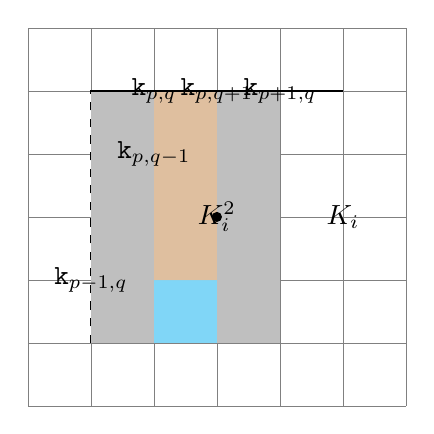
\begin{tikzpicture}[scale=0.8]
        % Draw the grid
        \draw[help lines] (0,0) grid (6,6);
        
        % Define coordinates for the elements
        \coordinate (A) at (1,1);
        \coordinate (B) at (2,1);
        \coordinate (C) at (3,1);
        \coordinate (D) at (4,1);
        \coordinate (E) at (5,1);
        \coordinate (F) at (1,2);
        \coordinate (G) at (2,2);
        \coordinate (H) at (3,2);
        \coordinate (I) at (4,2);
        \coordinate (J) at (5,2);
        \coordinate (K) at (1,3);
        \coordinate (L) at (2,3);
        \coordinate (M) at (3,3);
        \coordinate (N) at (4,3);
        \coordinate (O) at (5,3);
        \coordinate (P) at (1,4);
        \coordinate (Q) at (2,4);
        \coordinate (R) at (3,4);
        \coordinate (S) at (4,4);
        \coordinate (T) at (5,4);
        \coordinate (U) at (1,5);
        \coordinate (V) at (2,5);
        \coordinate (W) at (3,5);
        \coordinate (X) at (4,5);
        \coordinate (Y) at (5,5);
        
        % Draw the dashed border for K_i^2
        \draw[dashed] (A) rectangle (D |- Y);
        
        % Fill the coarse element K_i^2 with gray
        \fill[gray!50] (A) rectangle (D |- Y);
        
        % Fill the fine element k_{p,q} with blue
        \fill[cyan!50] (B) rectangle (C |- Y);
        
        % Fill the fine elements around K_i^2 with gray
        \fill[gray!50] (A |- F) rectangle (D |- J);
        \fill[gray!50] (A |- K) rectangle (D |- M);
        \fill[gray!50] (A |- P) rectangle (D |- S);
        
        % Fill the fine elements above K_i^2 with gray
        \fill[gray!50] (A |- F) rectangle (B |- Y);
        \fill[gray!50] (C |- F) rectangle (D |- Y);
        
        % Fill the fine elements below K_i^2 with gray
        \fill[gray!50] (A |- P) rectangle (B |- Y);
        \fill[gray!50] (C |- P) rectangle (D |- Y);
        
        % Fill the fine element in the top-left corner with brown
        \fill[brown!50] (B |- F) rectangle (C |- Y);
        
        % Label the elements
        \node at (B |- Y) {$\mathtt{k}_{p,q}$};
        \node at (A |- F) {$\mathtt{k}_{p-1,q}$};
        \node at (D |- Y) {$\mathtt{k}_{p+1,q}$};
        \node at (B |- P) {$\mathtt{k}_{p,q-1}$};
        \node at (C |- Y) {$\mathtt{k}_{p,q+1}$};
        \node at (3, 3) {$K_i^2$};
        \node at (5, 3) {$K_i$};
        
        % Draw the black vertical line
        \draw[line width=1pt] (D |- Y) -- (D |- Y |- Y);
        
        % Draw the black horizontal line
        \draw[line width=1pt] (A |- Y) -- (E |- Y);
        
        % Draw the black dot
        \filldraw[black] (3, 3) circle (2pt);
    \end{tikzpicture}
    \caption{An illustration for the proof of \cref{lem:A_i}, where $\mathtt{k}_{p,q}$, $\mathtt{k}_{p-1,q}$, $\mathtt{k}_{p+1,q}$, $\mathtt{k}_{p,q-1}$ and $\mathtt{k}_{p,q+1}$ are values of $\kappa$ on the fine elements respectively, the oversampling coarse element $K_i^m$ with $m=2$ is filled with gray and also decorated with dashed borderlines, and the fine element in the top-left corner of $K_i^m$ is highlighted.}
    \label{fig:illustration}
\end{figure}

\end{document}